\section{Compound Frequency Models}
\label{sect:cpd-freq-model}
\subsection{Compound Frequency Distributions}
\begin{enumerate}
\item Apart from mixing discussed in \cref{sect:mixing-and-ce}, another method
to create a new discrete distribution is to \emph{compound} (\faIcon{not-equal}
mix!) two discrete distributions.

\item \label{it:cpd-dist-s}
Let \(P_N\) and \(P_M\) be the pgf of the discrete random variables \(N\)
and \(M\) respectively. Then, define a new function \(P_S\) by
\[
P_S(t)=P_N(P_M(t)).
\]
Consider a random variable \(S\) with pgf \(P_S\). The distribution of \(S\) is
called a \defn{compound distribution} (and \(S\) is called \defn{compound
random variable}), where:
\begin{itemize}
\item distribution of \(N\) is called \defn{primary distribution} (\faIcon{arrows-alt-h} outer pgf);
\item distribution of \(M\) is called \defn{secondary distribution} (\faIcon{arrows-alt-h} inner pgf).
\end{itemize}
\begin{mnemonic}
Output from the pgf of \emph{secondary} distribution is fed into the pgf of
\emph{primary} distribution:
\begin{center}
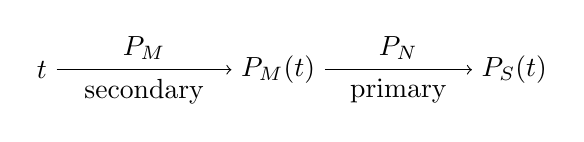
\begin{tikzpicture}
\node[] (t) at (0,0) {\(t\)};
\node[] (pm) at (3,0) {\(P_M(t)\)};
\node[] (ps) at (6,0) {\(P_S(t)\)};
\draw[->] (t) -- (pm) node[midway, above]{\(P_M\)} node[midway, below]{secondary};
\draw[->] (pm) -- (ps) node[midway, above]{\(P_N\)} node[midway, below]{primary};
\end{tikzpicture}
\end{center}
\end{mnemonic}
\item \label{it:cpd-dist-as-total-claims}
A practical interpretation of \(S\) is as follows. Let:
\begin{itemize}
\item \(N\): number of accidents arising in a portfolio of risks, with pgf \(P_N\)
\item \(M_1,M_2,\dotsc\): number of claims from each accident
\item \(S\): total number of claims
\end{itemize}
Then, \(S=M_1+\dotsb+M_N\).

\begin{remark}
\item The number of summands is \(N\), a random variable.
\item The equation \(S=M_1+\dotsb+M_N\) means that given
\(N={\color{violet}n}\), we have \(S=M_1+\dotsb+M_{\color{violet}n}\).
\end{remark}
\begin{theorem}
\label{thm:equiv-def-cpd-dist}
Suppose that \(M_1,M_2,\dotsc\) are i.i.d.\ (with the same distribution as
random variable \(M\)) and are independent of \(N\). The pgf of \(S\) is
\[
P_S(t)=P_N(P_M(t)).
\]
\begin{note}
This suggests that the definition of compound distribution using pgf (in
\labelcref{it:cpd-dist-s}) and using sum of \(N\) i.i.d.\ random variables
(here) are equivalent (in the sense that both result in the same distribution).
\end{note}
\end{theorem}
\begin{pf}
Note that
\begin{align*}
P_S(t)&=\sum_{k=0}^{\infty}t^k{\color{violet}\prob{S=k}}\\
&=\sum_{k=0}^{\infty}t^k{\color{violet}\sum_{n=0}^{\infty}\prob{S=k|N=n}\prob{N=n}}\\
&=\sum_{n=0}^{\infty}\prob{N=n}\sum_{k=0}^{\infty}t^k\prob{M_1+\dotsb+M_n=k|N=n}\\
&=\sum_{n=0}^{\infty}\prob{N=n}{\color{orange}\sum_{k=0}^{\infty}t^k\prob{M_1+\dotsb+M_n=k}}&\text{(by independence)}\\
&=\sum_{n=0}^{\infty}\prob{N=n}{\color{orange}P_{M_1+\dotsb+M_n}(t)}\\
&=\sum_{n=0}^{\infty}\prob{N=n}[P_{M}(t)]^n&\text{(\cref{prp:pgf-sum}, i.i.d.\ assumption)}\\
&=\expv{[P_M(t)]^N}\\
&=P_N(P_M(t)).
\end{align*}
\begin{note}
\(P_{M_1+\dotsb+M_n}\) and \(P_M\) are the pgf's of \(M_1+\dotsb+M_n\) and
\(M\) respectively.
\end{note}
\end{pf}

\item \label{it:cpd-dist-mean-var}
Consider the setting in \labelcref{it:cpd-dist-s}. The mean and variance of
\(S\) are as follows.
\begin{itemize}
\item \(\expv{S}=\expv{N}\expv{M}\)
\item \(\vari{S}=\expv{N}\vari{M}+(\expv{M})^2\vari{N}\)
\end{itemize}
\begin{pf}
We shall use the equivalent definition suggested by
\cref{thm:equiv-def-cpd-dist} to prove these formulas.

Firstly, note that
\[
\expv{S|N=n}=\expv{M_1+\dotsb+M_N|N=n}
=\expv{M_1+\dotsb+M_n|N=n}=\expv{M_1+\dotsb+M_n}
=n\expv{M}.
\]
Hence, \(\expv{S|N}=N\expv{M}\). Thus, by law of total expectation,
\[
\expv{S}=\expv{\expv{S|N}}
=\expv{N{\color{violet}\expv{M}}}
={\color{violet}\expv{M}}\expv{N}.
\]
Next, for the variance formula, first consider:
\begin{align*}
\vari{S|N=n}
&=\vari{M_1+\dotsb+M_N|N=n} \\
&=\vari{M_1+\dotsb+M_n|N=n} \\
&=\vari{M_1+\dotsb+M_n} &\text{(by independence)}\\
&=n\vari{M}&\text{(i.i.d.\ assumption)}.
\end{align*}
Thus, \(\vari{S|N}=N\vari{M}\), and by law of total variance,
\[
\vari{S}=\expv{\vari{S|N}}+\vari{\expv{S|N}}
=\expv{N{\color{violet}\vari{M}}}+\vari{N{\color{orange}\expv{M}}}
={\color{violet}\vari{M}}\expv{N}+{\color{orange}(\expv{M})^2}\vari{N}.
\]
\end{pf}
\end{enumerate}
\subsection{Panjer's Recursion}
\begin{enumerate}
\item Consider again the setting in \labelcref{it:cpd-dist-s}. Let:
\begin{itemize}
\item \(g_k=\prob{S=k}\);
\item \(p_k=\prob{N=k}\);
\item \(f_k=\prob{M=k}\).
\end{itemize}
Suppose that \(p_k\) and \(f_k\) are known for any \(k\ge 0\). Then, we are
interested in finding the distribution of \(S\), i.e., the value of \(g_k\) for
any \(k\ge 0\). Unfortunately, in general there is no simple way to do this.

\item However, in the special case where \(N\) is in the \((a,b,0)\) class, we
have the following result that allows us to compute \(g_k\) recursively.
\begin{theorem}[Panjer's recursion (\((a,b,0)\) class)]
\label{thm:panjer-recursion-ab0}
In this special case, for any \(k\ge 1\) (in the support of \(S\)),
\[
{\color{violet}g_k}=\frac{1}{1-af_0}\sum_{j=1}^{k}\qty(a+\frac{bj}{k})f_j{\color{violet}g_{k-j}}.
\]
\end{theorem}
\begin{pf}
Omitted (See, e.g., proof of theorem 7.1 in \textcite{klugman2019loss}).
\end{pf}

\begin{remark}
\item The \(a\) and \(b\) are the constants \(a\) and \(b\) in the \((a,b,0)\)
class characterization of \(S\).
\item To use the Panjer's recursion, we need the initial value \(g_0\). It can be
obtained by
\[
g_0=P_S(0)=P_N(P_M(0))=P_N(f_0).
\]
\item Some special cases:
\begin{itemize}
\item (\(k=1\)) \(\displaystyle g_1=\frac{1}{1-af_0}\qty(a+\frac{b\cdot 1}{1})f_1g_0\)
\item (\(k=2\)) \(\displaystyle g_2=\frac{1}{1-af_0}\qty[\qty(a+\frac{b\cdot 1}{2})f_1g_1
+\qty(a+\frac{b\cdot 2}{2}f_2g_0)]\)
\item (\(k=3\)) \(\displaystyle g_3=\frac{1}{1-af_0}\qty[\qty(a+\frac{b\cdot 1}{3})f_1g_2
+\qty(a+\frac{b\cdot 2}{3}f_2g_1)+\qty(a+\frac{b\cdot 3}{3}f_3g_0)
]\)
\end{itemize}
\end{remark}
\item When \(N\) is in the \((a,b,1)\) class instead, we can slightly
modify the Panjer's recursion to obtain the appropriate recursive formula as
follows.
\begin{theorem}[Panjer's recursion (\((a,b,1)\) class)]
\label{thm:panjer-recursion-ab1}
In this special case, for any \(k\ge 1\),
\[
{\color{violet}g_k}=\frac{1}{1-af_0}\qty{{\color{orange}[p_1-(a+b)p_0]f_k}+
\sum_{j=1}^{k}\qty(a+\frac{bj}{k})f_j{\color{violet}g_{k-j}}}.
\]
\end{theorem}
\begin{pf}
Similar to the proof for \cref{thm:panjer-recursion-ab0}.
\end{pf}
\end{enumerate}
\subsection{Compound Poisson Frequency Distributions}
\begin{enumerate}
\item If \(S\) is a compound random variable with the \emph{primary}
distribution being \(\pois{\lambda}\), then \(S\) follows a \defn{compound
Poisson distribution} (and \(S\) is called a \defn{compound Poisson random
variable}).

\item \label{it:cpd-pois-pgf}
Recall from \labelcref{it:pois-pgf} that the pgf of
\(N\sim\pois{\lambda}\) is
\[
P_N({\color{violet}s})=\exp{\lambda({\color{violet}s}-1)}.
\]
Thus, the pgf of a compound Poisson random variable \(S\) is
\[
P_S(t)=P_N({\color{violet}P_M(t)})=\boxed{\exp{\lambda({\color{violet}P_M(t)}-1)}}
\]
where \(P_M\) is the pgf for the secondary distribution.

\item \label{it:pgf-expr-for-cpd-pois}
Conversely, if \(S\) is a discrete random variable whose pgf can be
expressed as
\[
P_S(t)=\exp{\lambda(Q(t)-1)}
\]
for some function \(Q\) which serves as a pgf of a discrete random variable,
then \(S\) is a compound Poisson random variable with primary distribution
being \(\pois{\lambda}\) and secondary distribution identified by the pgf
\(Q\).

\begin{note}
This holds since same pgf implies same distribution, by
\cref{cor:pgf-equal-dist}.
\end{note}

\item Recall the convolution result for Poisson distribution
(\cref{thm:pois-convolution}). It turns out that analogous result holds also
for \emph{compound} Poisson distribution:

\begin{theorem}
\label{thm:cpd-pois-convolution}
Let \(S_1,\dotsc,S_k\) be \(k\) independent compound Poisson random variables
with Poisson parameters \(\lambda_1,\dotsc,\lambda_k\) respectively. Suppose
that the pmf of the secondary distribution for \(S_i\) is given by \(q_i(n)\),
for any \(i=1,\dotsc,k\). Then, the sum \(S=S_1+\dotsb+S_k\) is also a compound
Poisson random variable with Poisson parameter
\(\lambda=\lambda_1+\dotsb+\lambda_k\), and the pmf of the secondary
distribution is given by
\[
q(n)=\frac{\lambda_1}{\lambda}q_1(n)+\dotsb+\frac{\lambda_k}{\lambda}q_k(n).
\]
\begin{note}
\(q(n)\) is a legitimate pmf since \(q(n)\ge 0\) (as \(q_1(n),\dotsc,q_k(n)\ge
0\)) for any \(n\in\N_0\) and
\[
\sum_{n=0}^{\infty}q(n)=\frac{\lambda_1}{\lambda}\sum_{n=0}^{\infty}q_1(n)+\dotsb+
\frac{\lambda_k}{\lambda}\sum_{n=0}^{\infty}q_k(n)
=\frac{\lambda_1+\dotsb+\lambda_k}{\lambda}=1.
\]
\end{note}
\end{theorem}
\begin{pf}
Let \(Q_i\) be the pgf of the secondary distribution for \(S_i\), i.e.,
\[
Q_i(t)=\sum_{n=0}^{\infty}t^nq_i(n).
\]
Then, for any \(i=1,\dotsc,k\), the pgf of \(S_i\) can be expressed as
\[
P_{S_i}(t)=\exp{\lambda_i(Q_i(t)-1)}.
\]
Also, the pgf of the secondary distribution for \(S\) is
\[
Q(t)=\sum_{n=0}^{\infty}t^nq(n)
=\frac{\lambda_1}{\lambda}\sum_{n=0}^{\infty}t^nq_1(n)
+\dotsb+\frac{\lambda_k}{\lambda}\sum_{n=0}^{\infty}t^nq_k(n)
=\frac{\lambda_1}{\lambda}Q_1(t)+\dotsb+\frac{\lambda_k}{\lambda}Q_k(t).
\]

Since \(S_1,\dotsc,S_k\) are independent, by \cref{prp:pgf-sum}, the pgf of
\(S\) is
\[
P_S(t)=\prod_{i=1}^{k}P_{S_i}(t)
=\prod_{i=1}^{k}\exp{\lambda_i(Q_i(t)-1)}
=\exp{\sum_{i=1}^{k}\lambda_iQ_i(t)-\sum_{i=1}^{k}\lambda_i}
=\exp{\lambda(Q(t)-1)}.
\]
Thus, the result follows by \labelcref{it:pgf-expr-for-cpd-pois}.
\end{pf}
\end{enumerate}
